% !TeX root = RJwrapper.tex
\title{konfound}
\author{by Joshua M. Rosenberg, Ran Xu, Kenneth A. Frank}

\maketitle

\abstract{%
An abstract of less than 150 words.
}

% Any extra LaTeX you need in the preamble

\hypertarget{introduction}{%
\subsection{Introduction}\label{introduction}}

In social science (and educational) research, we often wish to
understand how robust inferences about effects are to unobserved (or
controlled for) covariates, possible problems with measurement, and
other sources of bias. The goal of \texttt{konfound} is to carry out
sensitivity analysis to help analysts to \emph{quantify how robust
inferences are to potential sources of bias}. This package provides
functions based on developments in sensitivity analysis by Frank and
colleagues, which previously have been implemented in \texttt{Stata} and
through an Excel spreadsheet, in \texttt{R} through the
\texttt{konfound} package.

\hypertarget{background-on-sensitivity-analysis}{%
\section{Background on sensitivity
analysis}\label{background-on-sensitivity-analysis}}

\hypertarget{impact-threshold-of-a-confounding-variable}{%
\subsection{Impact threshold of a confounding
variable}\label{impact-threshold-of-a-confounding-variable}}

\hypertarget{percent-bias-to-invalidate-an-inference}{%
\subsection{Percent bias to invalidate an
inference}\label{percent-bias-to-invalidate-an-inference}}

\hypertarget{tutorial}{%
\section{Tutorial}\label{tutorial}}

You can install \texttt{konfound} with the following:

\begin{Schunk}
\begin{Sinput}
install.packages("konfound")
\end{Sinput}
\end{Schunk}

You can then load konfound with the \texttt{library()} function:

\begin{Schunk}
\begin{Sinput}
library(konfound)
\end{Sinput}
\begin{Soutput}
#> Sensitivity analysis as described in Frank, Maroulis, Duong, and Kelcey (2013) and in Frank (2000).
#> For more information visit https://jmichaelrosenberg.shinyapps.io/shinykonfound/.
\end{Soutput}
\end{Schunk}

\hypertarget{use-of-pkonfound-for-values-from-an-already-conducted-analysis}{%
\subsection{Use of pkonfound() for values from an already-conducted
analysis}\label{use-of-pkonfound-for-values-from-an-already-conducted-analysis}}

\texttt{pkonfound()} is used when we have values from an
already-conducted analysis (like a regression analysis), such as one in
an already-published study or from an analysis carried out using other
software.

In the case of a regression analysis, values from the analysis would
simply be used as the inputs to the \texttt{pkonfound()} function. For
example, in the use below, we simply enter the values for the estimated
effect (an unstandardardized beta coefficient) (\texttt{2}), its
standard error (\texttt{.4}), the sample size (\texttt{100}), and the
number of covariates (\texttt{3}):

\begin{Schunk}
\begin{Sinput}
pkonfound(2, .4, 100, 3)
\end{Sinput}
\begin{Soutput}
#> Replacement of Cases Approach:
#> To invalidate an inference, 60.3% of the estimate would have to be due to
bias. This is based on a threshold of 0.794 for statistical significance (alpha
= 0.05).
#> To invalidate an inference, 60 observations would have to be replaced with
cases for which the effect is 0.
#>
#> Correlation-based Approach:
#> An omitted variable would have to be correlated at 0.568 with the outcome
and at 0.568 with the predictor of interest (conditioning on observed
covariates) to invalidate an inference based on a threshold of 0.201 for
statistical significance (alpha = 0.05).
#> Correspondingly the impact of an omitted variable (as defined in Frank 2000)
must be 0.568 X 0.568 = 0.323 to invalidate an inference.
\end{Soutput}
\begin{Soutput}
#> For other forms of output, change `to_return` to table, raw_output, thres_plot, or corr_plot.
\end{Soutput}
\begin{Soutput}
#> For models fit in R, consider use of konfound().
\end{Soutput}
\end{Schunk}

For this set of values, around 60\% would need to be false due to a
source of bias for the inference to be invalidated (based on statistical
significance and a p-value (or alpha) of .05), possible a very robust
effect. An omitted, confounding variable (sometimes referred to as a
covariate) would need to have an impact (defined as the product of the
confounding variable's correlation with both the predictor of interest
and the outcome) of 0.323, presenting a different interpretation of how
robust this (hypothetical) effect is to a variable which is important
but not included in the analysis.

Here is another example, but one in which the unstandardized beta
coefficient is smaller than its standard error:

\begin{Schunk}
\begin{Sinput}
pkonfound(.4, 2, 100, 3)
\end{Sinput}
\begin{Soutput}
#> Replacement of Cases Approach:
#> To sustain an inference, 89.924% of the estimate would have to be due to
bias. This is based on a threshold of 3.97 for statistical significance (alpha
= 0.05).
#> To sustain an inference, 90 of the cases with 0 effect would have to be
replaced with cases at the threshold of inference.
#>
#> Correlation-based Approach:
#> An omitted variable would have to be correlated at 0.387 with the outcome
and at 0.387 with the predictor of interest (conditioning on observed
covariates) to sustain an inference based on a threshold of 3.97 for
statistical significance (alpha = 0.05).
#> Correspondingly the impact of an omitted variable (as defined in Frank 2000)
must be 0.387 X 0.387 = 0.15 to sustain an inference.
\end{Soutput}
\begin{Soutput}
#> For other forms of output, change `to_return` to table, raw_output, thres_plot, or corr_plot.
\end{Soutput}
\begin{Soutput}
#> For models fit in R, consider use of konfound().
\end{Soutput}
\end{Schunk}

Note that this use of \texttt{pkonfound()} is equivalent to naming the
arguments, i.e.~for a different set of values:

\begin{Schunk}
\begin{Sinput}
pkonfound(est_eff = -2.2,
          std_err = .65, 
          n_obs = 200,
          n_covariates = 3)
\end{Sinput}
\begin{Soutput}
#> Replacement of Cases Approach:
#> To invalidate an inference, 41.732% of the estimate would have to be due to
bias. This is based on a threshold of -1.282 for statistical significance
(alpha = 0.05).
#> To invalidate an inference, 83 observations would have to be replaced with
cases for which the effect is 0.
#>
#> Correlation-based Approach:
#> An omitted variable would have to be correlated at 0.334 with the outcome
and at 0.334 with the predictor of interest (conditioning on observed
covariates) to invalidate an inference based on a threshold of -0.14 for
statistical significance (alpha = 0.05).
#> Correspondingly the impact of an omitted variable (as defined in Frank 2000)
must be 0.334 X 0.334 = 0.112 to invalidate an inference.
\end{Soutput}
\begin{Soutput}
#> For other forms of output, change `to_return` to table, raw_output, thres_plot, or corr_plot.
\end{Soutput}
\begin{Soutput}
#> For models fit in R, consider use of konfound().
\end{Soutput}
\end{Schunk}

We notice that the output includes a message that says we can view other
forms of output by changing the \texttt{to\_return} argument. Here are
the two plots - for the bias necessary to alter an inference
(\texttt{thresh\_plot}) and for the robustness of an inference in terms
of the impact of a confounding variable (\texttt{corr\_plot}) that can
be returned:

\begin{Schunk}
\begin{Sinput}
pkonfound(.4, 2, 100, 3, to_return = "thresh_plot")
\end{Sinput}


\begin{center}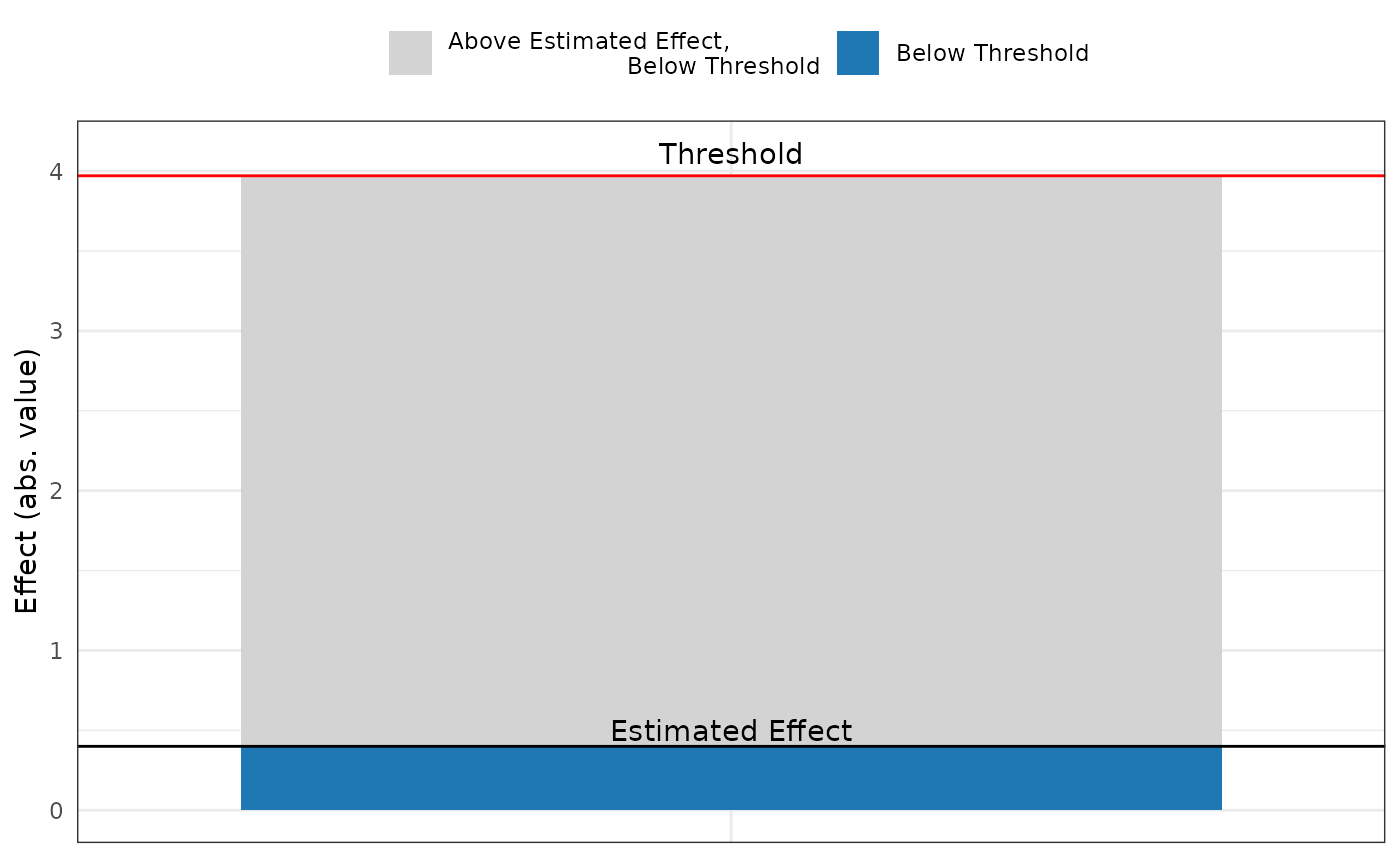
\includegraphics[width=0.7\linewidth]{konfound_files/figure-latex/unnamed-chunk-5-1} \end{center}

\end{Schunk}

\begin{Schunk}
\begin{Sinput}
pkonfound(.4, 2, 100, 3, to_return = "corr_plot")
\end{Sinput}


\begin{center}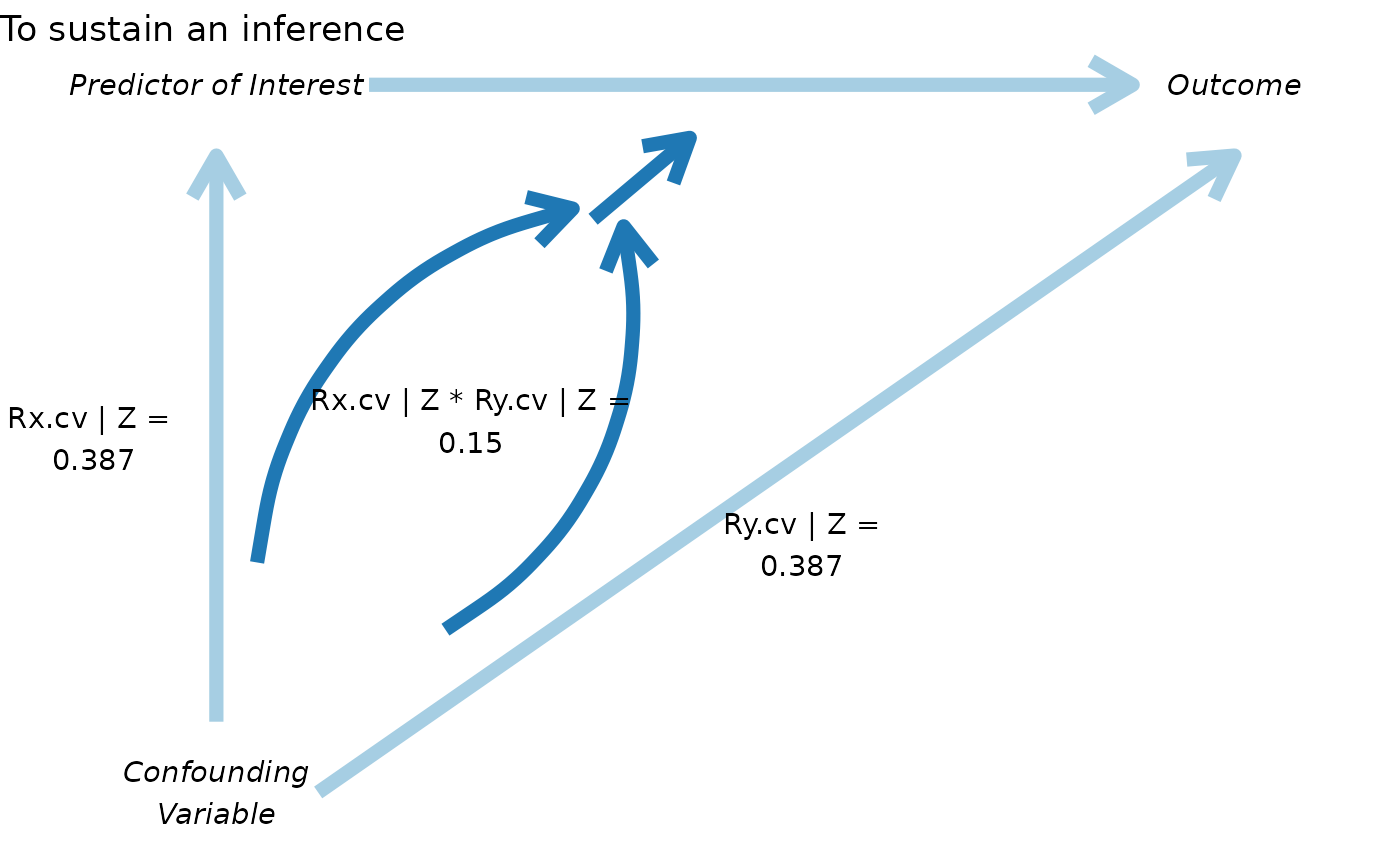
\includegraphics[width=0.7\linewidth]{konfound_files/figure-latex/unnamed-chunk-6-1} \end{center}

\end{Schunk}

You can also specify multiple forms of output at once.

\begin{Schunk}
\begin{Sinput}
model_output <- pkonfound(2, .4, 200, 3, to_return = c("raw_output", "thresh_plot", "corr_plot"))
\end{Sinput}
\begin{Soutput}
#> Replacement of Cases Approach:
#> To invalidate an inference, 60.557% of the estimate would have to be due to bias. This is based on a threshold of 0.789 for statistical significance (alpha = 0.05).
#> To invalidate an inference, 121 observations would have to be replaced with cases for which the effect is 0.
#> 
#> Correlation-based Approach:
#> An omitted variable would have to be correlated at 0.479 with the outcome and at 0.479 with the predictor of interest (conditioning on observed covariates) to invalidate an inference based on a threshold of 0.14 for statistical significance (alpha = 0.05).
#> Correspondingly the impact of an omitted variable (as defined in Frank 2000) must be 0.479 X 0.479 = 0.229 to invalidate an inference.
\end{Soutput}
\begin{Soutput}
#> Print output created by default. Created 3 other forms of output. Use list indexing or run summary() on the output to see how to access.
\end{Soutput}
\begin{Sinput}
summary(model_output)
\end{Sinput}
\begin{Soutput}
#> Created 3 forms of output. To access type: 
#> 
#> model_output$raw_output
#> model_output$thresh_plot
#> model_output$corr_plot
\end{Soutput}
\end{Schunk}

When we type the name of the object, we see that we created three types
of output that we can access as follows:

\begin{Schunk}
\begin{Sinput}
model_output$raw_output
\end{Sinput}
\begin{Soutput}
#> # A tibble: 1 x 8
#>   action inference percent_bias_to~ replace_null_ca~ unstd_beta
#>   <chr>  <chr>                <dbl>            <dbl>      <dbl>
#> 1 to_in~ reject_n~             60.6              121          2
#> # ... with 3 more variables: beta_threshhold <dbl>,
#> #   omitted_variable_corr <dbl>, itcv <dbl>
\end{Soutput}
\begin{Sinput}
model_output$thresh_plot
\end{Sinput}


\begin{center}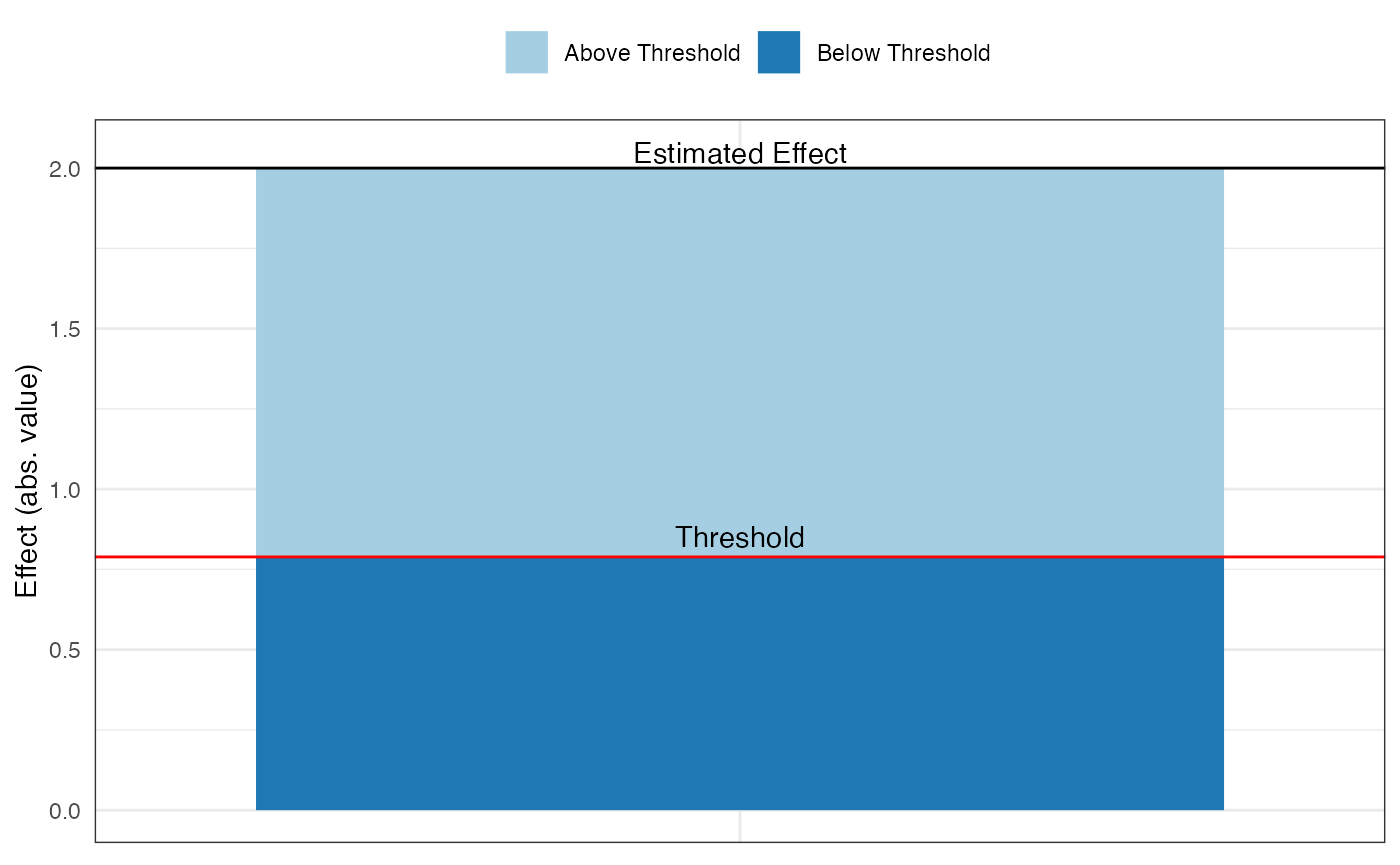
\includegraphics[width=0.7\linewidth]{konfound_files/figure-latex/unnamed-chunk-8-1} \end{center}

\begin{Sinput}
model_output$corr_plot
\end{Sinput}


\begin{center}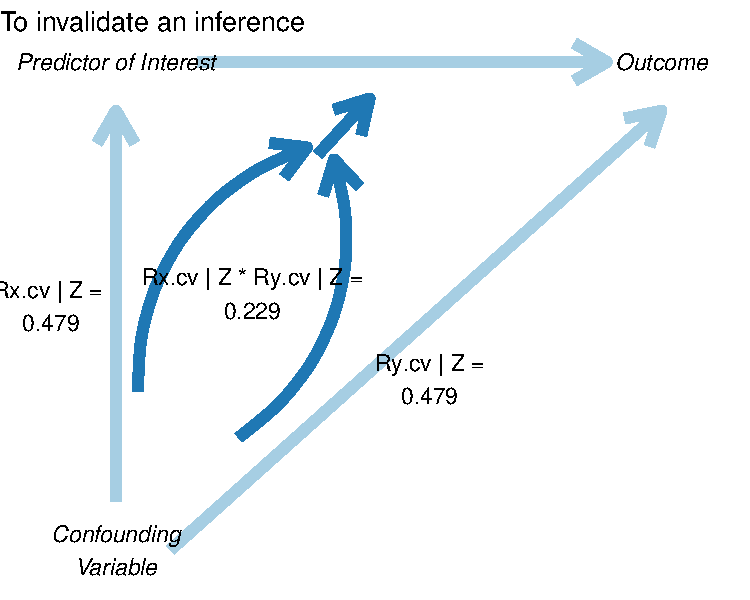
\includegraphics[width=0.7\linewidth]{konfound_files/figure-latex/unnamed-chunk-8-2} \end{center}

\end{Schunk}

Finally, you can return the raw output, for use in other analyses.

\begin{Schunk}
\begin{Sinput}
pkonfound(.4, 2, 100, 3, to_return = "raw_output")
\end{Sinput}
\begin{Soutput}
#> # A tibble: 1 x 8
#>   action inference percent_bias_to~ replace_null_ca~ unstd_beta
#>   <chr>  <chr>                <dbl>            <dbl>      <dbl>
#> 1 to_su~ fail_to_~             89.9               90        0.4
#> # ... with 3 more variables: beta_threshhold <dbl>,
#> #   omitted_variable_corr <dbl>, itcv <dbl>
\end{Soutput}
\end{Schunk}

\hypertarget{use-of-konfound-for-models-fit-in-r}{%
\subsection{Use of konfound() for models fit in
R}\label{use-of-konfound-for-models-fit-in-r}}

Where \texttt{pkonfound()} can be used with values from
already-conducted analyses, \texttt{konfound()} can be used with models
(\texttt{lm()}, \texttt{glm()}, and \texttt{lme4::lmer()}) fit in R.

\textbf{For linear models fit with lm()}

\begin{Schunk}
\begin{Sinput}
m1 <- lm(mpg ~ wt + hp + qsec, data = mtcars)
m1
\end{Sinput}
\begin{Soutput}
#> 
#> Call:
#> lm(formula = mpg ~ wt + hp + qsec, data = mtcars)
#> 
#> Coefficients:
#> (Intercept)           wt           hp         qsec  
#>    27.61053     -4.35880     -0.01782      0.51083
\end{Soutput}
\begin{Sinput}

konfound(m1, hp)
\end{Sinput}
\begin{Soutput}
#> Note that this output is calculated based on the correlation-based approach used in mkonfound()
\end{Soutput}
\begin{Soutput}
#> Replacement of Cases Approach:
#> To sustain an inference, 41.327% of the estimate would have to be due to bias. This is based on a threshold of -0.031 for statistical significance (alpha = 0.05).
#> To sustain an inference, 13 of the cases with 0 effect would have to be replaced with cases at the threshold of inference.
#> 
#> Correlation-based Approach:
#> An omitted variable would have to be correlated at 0.322 with the outcome and at 0.322 with the predictor of interest (conditioning on observed covariates) to sustain an inference based on a threshold of -0.031 for statistical significance (alpha = 0.05).
#> Correspondingly the impact of an omitted variable (as defined in Frank 2000) must be 0.322 X 0.322 = 0.104 to sustain an inference.
\end{Soutput}
\begin{Soutput}
#> For more detailed output, consider setting `to_return` to table
\end{Soutput}
\begin{Soutput}
#> To consider other predictors of interest, consider setting `test_all` to TRUE.
\end{Soutput}
\end{Schunk}

Like with \texttt{pkonfound()}, we can also output multiple forms of
output at once with \texttt{konfound()}:

\begin{Schunk}
\begin{Sinput}
konfound_output <- konfound(m1, hp, to_return = c("raw_output", "thresh_plot", "corr_plot"))
\end{Sinput}
\begin{Soutput}
#> Note that this output is calculated based on the correlation-based approach used in mkonfound()
\end{Soutput}
\begin{Soutput}
#> Replacement of Cases Approach:
#> To sustain an inference, 41.327% of the estimate would have to be due to bias. This is based on a threshold of -0.031 for statistical significance (alpha = 0.05).
#> To sustain an inference, 13 of the cases with 0 effect would have to be replaced with cases at the threshold of inference.
#> 
#> Correlation-based Approach:
#> An omitted variable would have to be correlated at 0.322 with the outcome and at 0.322 with the predictor of interest (conditioning on observed covariates) to sustain an inference based on a threshold of -0.031 for statistical significance (alpha = 0.05).
#> Correspondingly the impact of an omitted variable (as defined in Frank 2000) must be 0.322 X 0.322 = 0.104 to sustain an inference.
\end{Soutput}
\begin{Soutput}
#> Print output created by default. Created 3 other forms of output. Use list indexing or run summary() on the output to see how to access.
\end{Soutput}
\begin{Sinput}
summary(konfound_output)
\end{Sinput}
\begin{Soutput}
#> Created 3 forms of output. To access type: 
#> 
#> konfound_output$raw_output
#> konfound_output$thresh_plot
#> konfound_output$corr_plot
\end{Soutput}
\end{Schunk}

Again, we can type each of those, i.e.:

\begin{Schunk}
\begin{Sinput}
konfound_output$raw_output
\end{Sinput}
\begin{Soutput}
#> # A tibble: 1 x 8
#>   action inference percent_bias_to~ replace_null_ca~ unstd_beta
#>   <chr>  <chr>                <dbl>            <dbl>      <dbl>
#> 1 to_su~ fail_to_~             41.3               13     -0.018
#> # ... with 3 more variables: beta_threshhold <dbl>,
#> #   omitted_variable_corr <dbl>, itcv <dbl>
\end{Soutput}
\begin{Sinput}
konfound_output$thresh_plot
\end{Sinput}


\begin{center}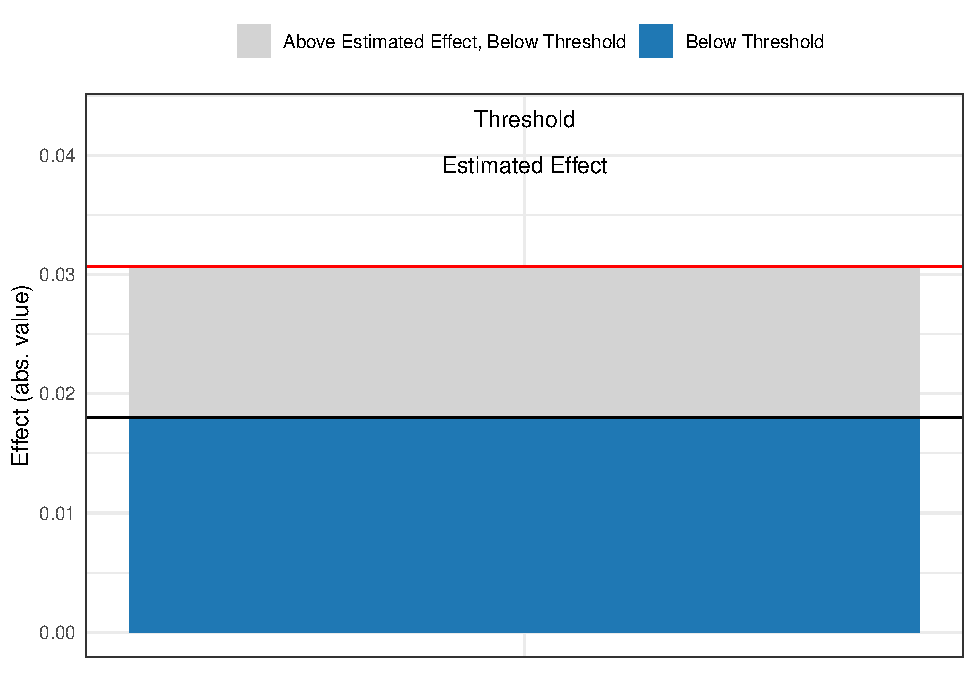
\includegraphics[width=0.7\linewidth]{konfound_files/figure-latex/unnamed-chunk-12-1} \end{center}

\end{Schunk}

We can also test all of the variables as predictors of interest:

\begin{Schunk}
\begin{Sinput}
konfound(m1, wt, test_all = TRUE)
\end{Sinput}
\begin{Soutput}
#> # A tibble: 3 x 8
#>   var_name     t    df action   inference  pct_bias_to_chang~   itcv r_con
#>   <chr>    <dbl> <dbl> <chr>    <chr>                   <dbl>  <dbl> <dbl>
#> 1 wt       -5.79    29 to_inva~ reject_nu~               51.5  0.585 0.765
#> 2 hp       -1.2     29 to_sust~ fail_to_r~               38.7 -0.102 0.319
#> 3 qsec      1.16    29 to_sust~ fail_to_r~               40.5 -0.106 0.326
\end{Soutput}
\end{Schunk}

Whereas this cannot be carried out with \texttt{pkonfound()}, with
\texttt{konfound()} you can also return a table with some key output
from the correlation-based approach.

\begin{Schunk}
\begin{Sinput}
konfound(m1, wt, to_return = "table")
\end{Sinput}
\begin{Soutput}
#> Note that this output is calculated based on the correlation-based approach used in mkonfound()
\end{Soutput}
\begin{Soutput}
#> Dependent variable is mpg
\end{Soutput}
\begin{Soutput}
#> Warning: Unknown or uninitialised column: 'itcv'.
\end{Soutput}
\begin{Soutput}
#> Warning: Unknown or uninitialised column: 'impact'.
\end{Soutput}
\begin{Soutput}
#> # A tibble: 4 x 7
#>   term        estimate std.error statistic p.value   itcv impact
#>   <chr>          <dbl>     <dbl>     <dbl>   <dbl>  <dbl>  <dbl>
#> 1 (Intercept)   27.6       8.42       3.28   0.003 NA     NA    
#> 2 wt            -4.36      0.753     -5.79   0      0.243 NA    
#> 3 hp            -0.018     0.015     -1.19   0.244 NA      0.511
#> 4 qsec           0.511     0.439      1.16   0.255 NA      0.073
\end{Soutput}
\end{Schunk}

If the impact threshhold is greater than the impacts of the \texttt{Z}s
(the other covariates) then an omitted variable would have to have a
greater impact than any of the observed covariates to change the
inference. Note that in fields in which there is a lot known about
covariates given the outcome of interest, then the omitted ones are
likely less important than those that are known an included (i.e., we
have a good sense of the factors that matter in terms of educational
achievement).

\textbf{For generalized linear models fit with glm()}

Effects for these models are interpreted on the basis of average partial
(or marginal) effects (calculated using the \texttt{margins} package).

\begin{Schunk}
\begin{Sinput}
# if forcats is not installed, this install it first using install.packages("forcats") for this to run
if (requireNamespace("forcats")) {
    d <- forcats::gss_cat
    
    d$married <- ifelse(d$marital == "Married", 1, 0)
    
    m2 <- glm(married ~ age, data = d, family = binomial(link = "logit"))
    konfound(m2, age)
}
\end{Sinput}
\begin{Soutput}
#> Replacement of Cases Approach:
#> To sustain an inference, 80.978% of the estimate would have to be due to bias. This is based on a threshold of 0.013 for statistical significance (alpha = 0.05).
#> To sustain an inference, 17334 of the cases with 0 effect would have to be replaced with cases at the threshold of inference.
#> 
#> Correlation-based Approach:
#> An omitted variable would have to be correlated at 5.535 with the outcome and at 5.535 with the predictor of interest (conditioning on observed covariates) to invalidate an inference based on a threshold of 1.003 for statistical significance (alpha = 0.05).
#> Correspondingly the impact of an omitted variable (as defined in Frank 2000) must be 5.535 X 5.535 = 30.636 to invalidate an inference.
\end{Soutput}
\begin{Soutput}
#> NULL
\end{Soutput}
\end{Schunk}

As with models fit with \texttt{lm()} (and use of \texttt{pkonfound()}),
multiple forms of output can be specified with the \texttt{to\_return}
argument to \texttt{konfound()}, i.e.
\texttt{konfound(m2,\ age,\ to\_return\ =\ c("raw\_output",\ "corr\_plot",\ "thresh\_plot"))}.

\textbf{For mixed effects (or multi-level) models fit with the lmer()
function from the lme4 package}

\texttt{konfound} also works with models fit with the \texttt{lmer()}
function from the package \texttt{lme4}, for mixed-effects or
multi-level models. One challenge with carrying out sensitivity analysis
for fixed effects in mixed effects models is calculating the correct
denominator degrees of freedom for the t-test associated with the
coefficients. This is not unique to sensitivity analysis, as, for
example, \texttt{lmer()} does not report degrees of freedom (or
p-values) for fixed effects predictors (see this information in the
\texttt{lme4} FAQ
\href{http://bbolker.github.io/mixedmodels-misc/glmmFAQ.html\#why-doesnt-lme4-display-denominator-degrees-of-freedomp-values-what-other-options-do-i-have}{here}).
While it may be possible to determine the correct degrees of freedom for
some models (i.e., models with relatively simple random effects
structures), it is difficult to generalize this approach, and so in this
package the Kenward-Roger approximation for the denominator degrees of
freedom as implemented in the \texttt{pbkrtest} package (described in
\href{https://www.jstatsoft.org/htaccess.php?volume=59\&type=i\&issue=09\&paper=true}{Halekoh
and Højsgaard, 2014}).

Here is an example of the use of \texttt{konfound()} with a model fit
with \texttt{lmer()}:

\begin{Schunk}
\begin{Sinput}
if (requireNamespace("lme4")) {
    library(lme4)
    m3 <- fm1 <- lmer(Reaction ~ Days + (1 | Subject), sleepstudy)
    konfound(m3, Days)
}
\end{Sinput}
\begin{Soutput}
#> Loading required namespace: lme4
\end{Soutput}
\begin{Soutput}
#> Loading required package: Matrix
\end{Soutput}
\begin{Soutput}
#> Warning in bind_rows_(x, .id): binding factor and character vector,
#> coercing into character vector
\end{Soutput}
\begin{Soutput}
#> Warning in bind_rows_(x, .id): binding character and factor vector,
#> coercing into character vector
\end{Soutput}
\begin{Soutput}
#> Replacement of Cases Approach:
#> To invalidate an inference, 84.83% of the estimate would have to be due to bias. This is based on a threshold of 1.588 for statistical significance (alpha = 0.05).
#> To invalidate an inference, 137 observations would have to be replaced with cases for which the effect is 0.
#> 
#> Correlation-based Approach:
#> An omitted variable would have to be correlated at 0.817 with the outcome and at 0.817 with the predictor of interest (conditioning on observed covariates) to invalidate an inference based on a threshold of 0.155 for statistical significance (alpha = 0.05).
#> Correspondingly the impact of an omitted variable (as defined in Frank 2000) must be 0.817 X 0.817 = 0.667 to invalidate an inference.
\end{Soutput}
\begin{Soutput}
#> Note that the Kenward-Roger approximation is used to estimate degrees of freedom for the predictor(s) of interest.
\end{Soutput}
\begin{Soutput}
#> NULL
\end{Soutput}
\end{Schunk}

\hypertarget{use-of-mkonfound-for-meta-analyses-that-include-sensitivity-analysis}{%
\subsection{Use of mkonfound() for meta-analyses that include
sensitivity
analysis}\label{use-of-mkonfound-for-meta-analyses-that-include-sensitivity-analysis}}

We can also use \texttt{konfound} to carry out sensitivity analysis as
part of meta-analyses. For example, here, \texttt{d} represents output
from a number (30 in this case) of past studies, read in a CSV file from
a website:

\begin{Schunk}
\begin{Sinput}
d <- read.csv("https://msu.edu/~kenfrank/example%20dataset%20for%20mkonfound.csv")
head(d)
\end{Sinput}
\begin{Soutput}
#>           t  df
#> 1  7.076763 178
#> 2  4.127893 193
#> 3  1.893137  47
#> 4 -4.166395 138
#> 5 -1.187599  97
#> 6  3.585478  87
\end{Soutput}
\begin{Sinput}
mkonfound(d, t, df)
\end{Sinput}
\begin{Soutput}
#> # A tibble: 30 x 7
#>         t    df action    inference      pct_bias_to_change_~   itcv r_con
#>     <dbl> <int> <chr>     <chr>                         <dbl>  <dbl> <dbl>
#>  1  7.08    178 to_inval~ reject_null                   68.8   0.378 0.614
#>  2  4.13    193 to_inval~ reject_null                   50.6   0.168 0.41 
#>  3  1.89     47 to_susta~ fail_to_rejec~                 5.47 -0.012 0.11 
#>  4 -4.17    138 to_inval~ reject_null                   50.3   0.202 0.449
#>  5 -1.19     97 to_susta~ fail_to_rejec~                39.4  -0.065 0.255
#>  6  3.59     87 to_inval~ reject_null                   41.9   0.19  0.436
#>  7  0.282   117 to_susta~ fail_to_rejec~                85.5  -0.131 0.361
#>  8  2.55     75 to_inval~ reject_null                   20.6   0.075 0.274
#>  9 -4.44    137 to_inval~ reject_null                   53.0   0.225 0.475
#> 10 -2.05    195 to_inval~ reject_null                    3.51  0.006 0.077
#> # ... with 20 more rows
\end{Soutput}
\end{Schunk}

We can also return a plot summarizing the percent bias needed to sustan
or invalidate an inference across all of the past studies:

\begin{Schunk}
\begin{Sinput}
mkonfound(d, t, df, return_plot = T)
\end{Sinput}
\begin{Soutput}
#> `stat_bin()` using `bins = 30`. Pick better value with `binwidth`.
\end{Soutput}


\begin{center}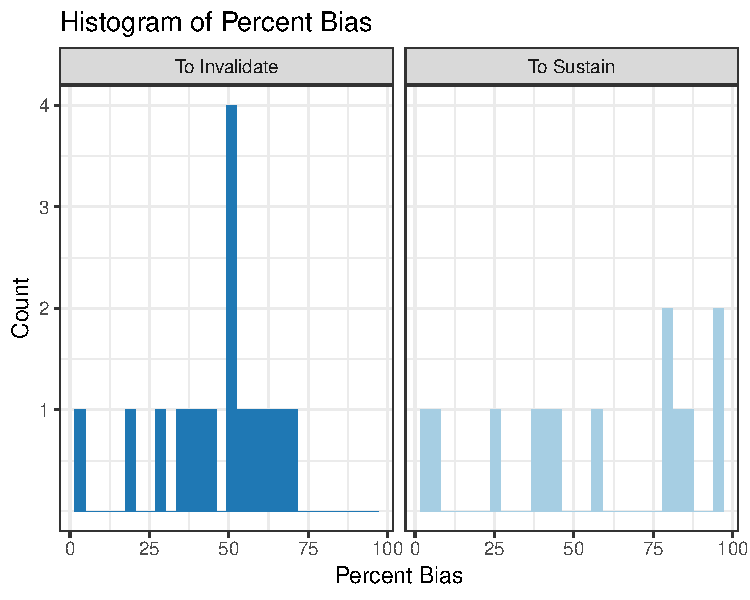
\includegraphics[width=0.7\linewidth]{konfound_files/figure-latex/unnamed-chunk-18-1} \end{center}

\end{Schunk}


\address{%
Joshua M. Rosenberg\\
University of Tennessee, Knoxville\\
line 1\\ line 2\\
}
\href{mailto:jmrosenberg@utk.edu}{\nolinkurl{jmrosenberg@utk.edu}}

\address{%
Ran Xu\\
Virginia Tech\\
line 1\\ line 2\\
}
\href{mailto:ranxu@msu.edu}{\nolinkurl{ranxu@msu.edu}}

\address{%
Kenneth A. Frank\\
Michigan State University\\
line 1\\ line 2\\
}
\href{mailto:kenfrank@msu.edu}{\nolinkurl{kenfrank@msu.edu}}

